\section{Soution methods}

\subsection{Value Function Iteration}

As a benchmark solution, I solve the problem by using value function iteration. However modifications to the algorithm presented in section \ref{sec:dynamic_programming}. First and foremost, i consider the Q-function instead of the value function, allowing to store state-action value pairs. Second it should be noted that in this formulation multiple of the features are continuous, not allowing for tabular solutions. Thirdly, the dimension of the state-space + the size of the grid made in infeasable\footnote{In my initial attempt to solve the model by value function iteration, i attempted to get the expectation of the value function using Gauss-Hermite integration, and discretizing the statespace. The solution time was infeasible, which was why my approach changed.} to solve the model by classical ways of solving a model using backwards induction an discreetizing the state space. 

The model is solved using backwards induction. This is due to the fact the model terminates in a deterministic fashion when the agents reaches a certain age. For each step a large random sample of states is drawn conditional on a given age. For each of these state the agent takes each of the possible actions storing the results. This way a large sample of rewards and states can be generated. Furthermore for each action taken (if the state is not terminal) the the Q-function can be evaluated in the new state, taken the max of each possible action, allowing for the estimation of the value function. A graphical representation of the concept is shown in figure \ref{fig:vfi_figure}. 

\begin{figure}[ht]
    \centering
    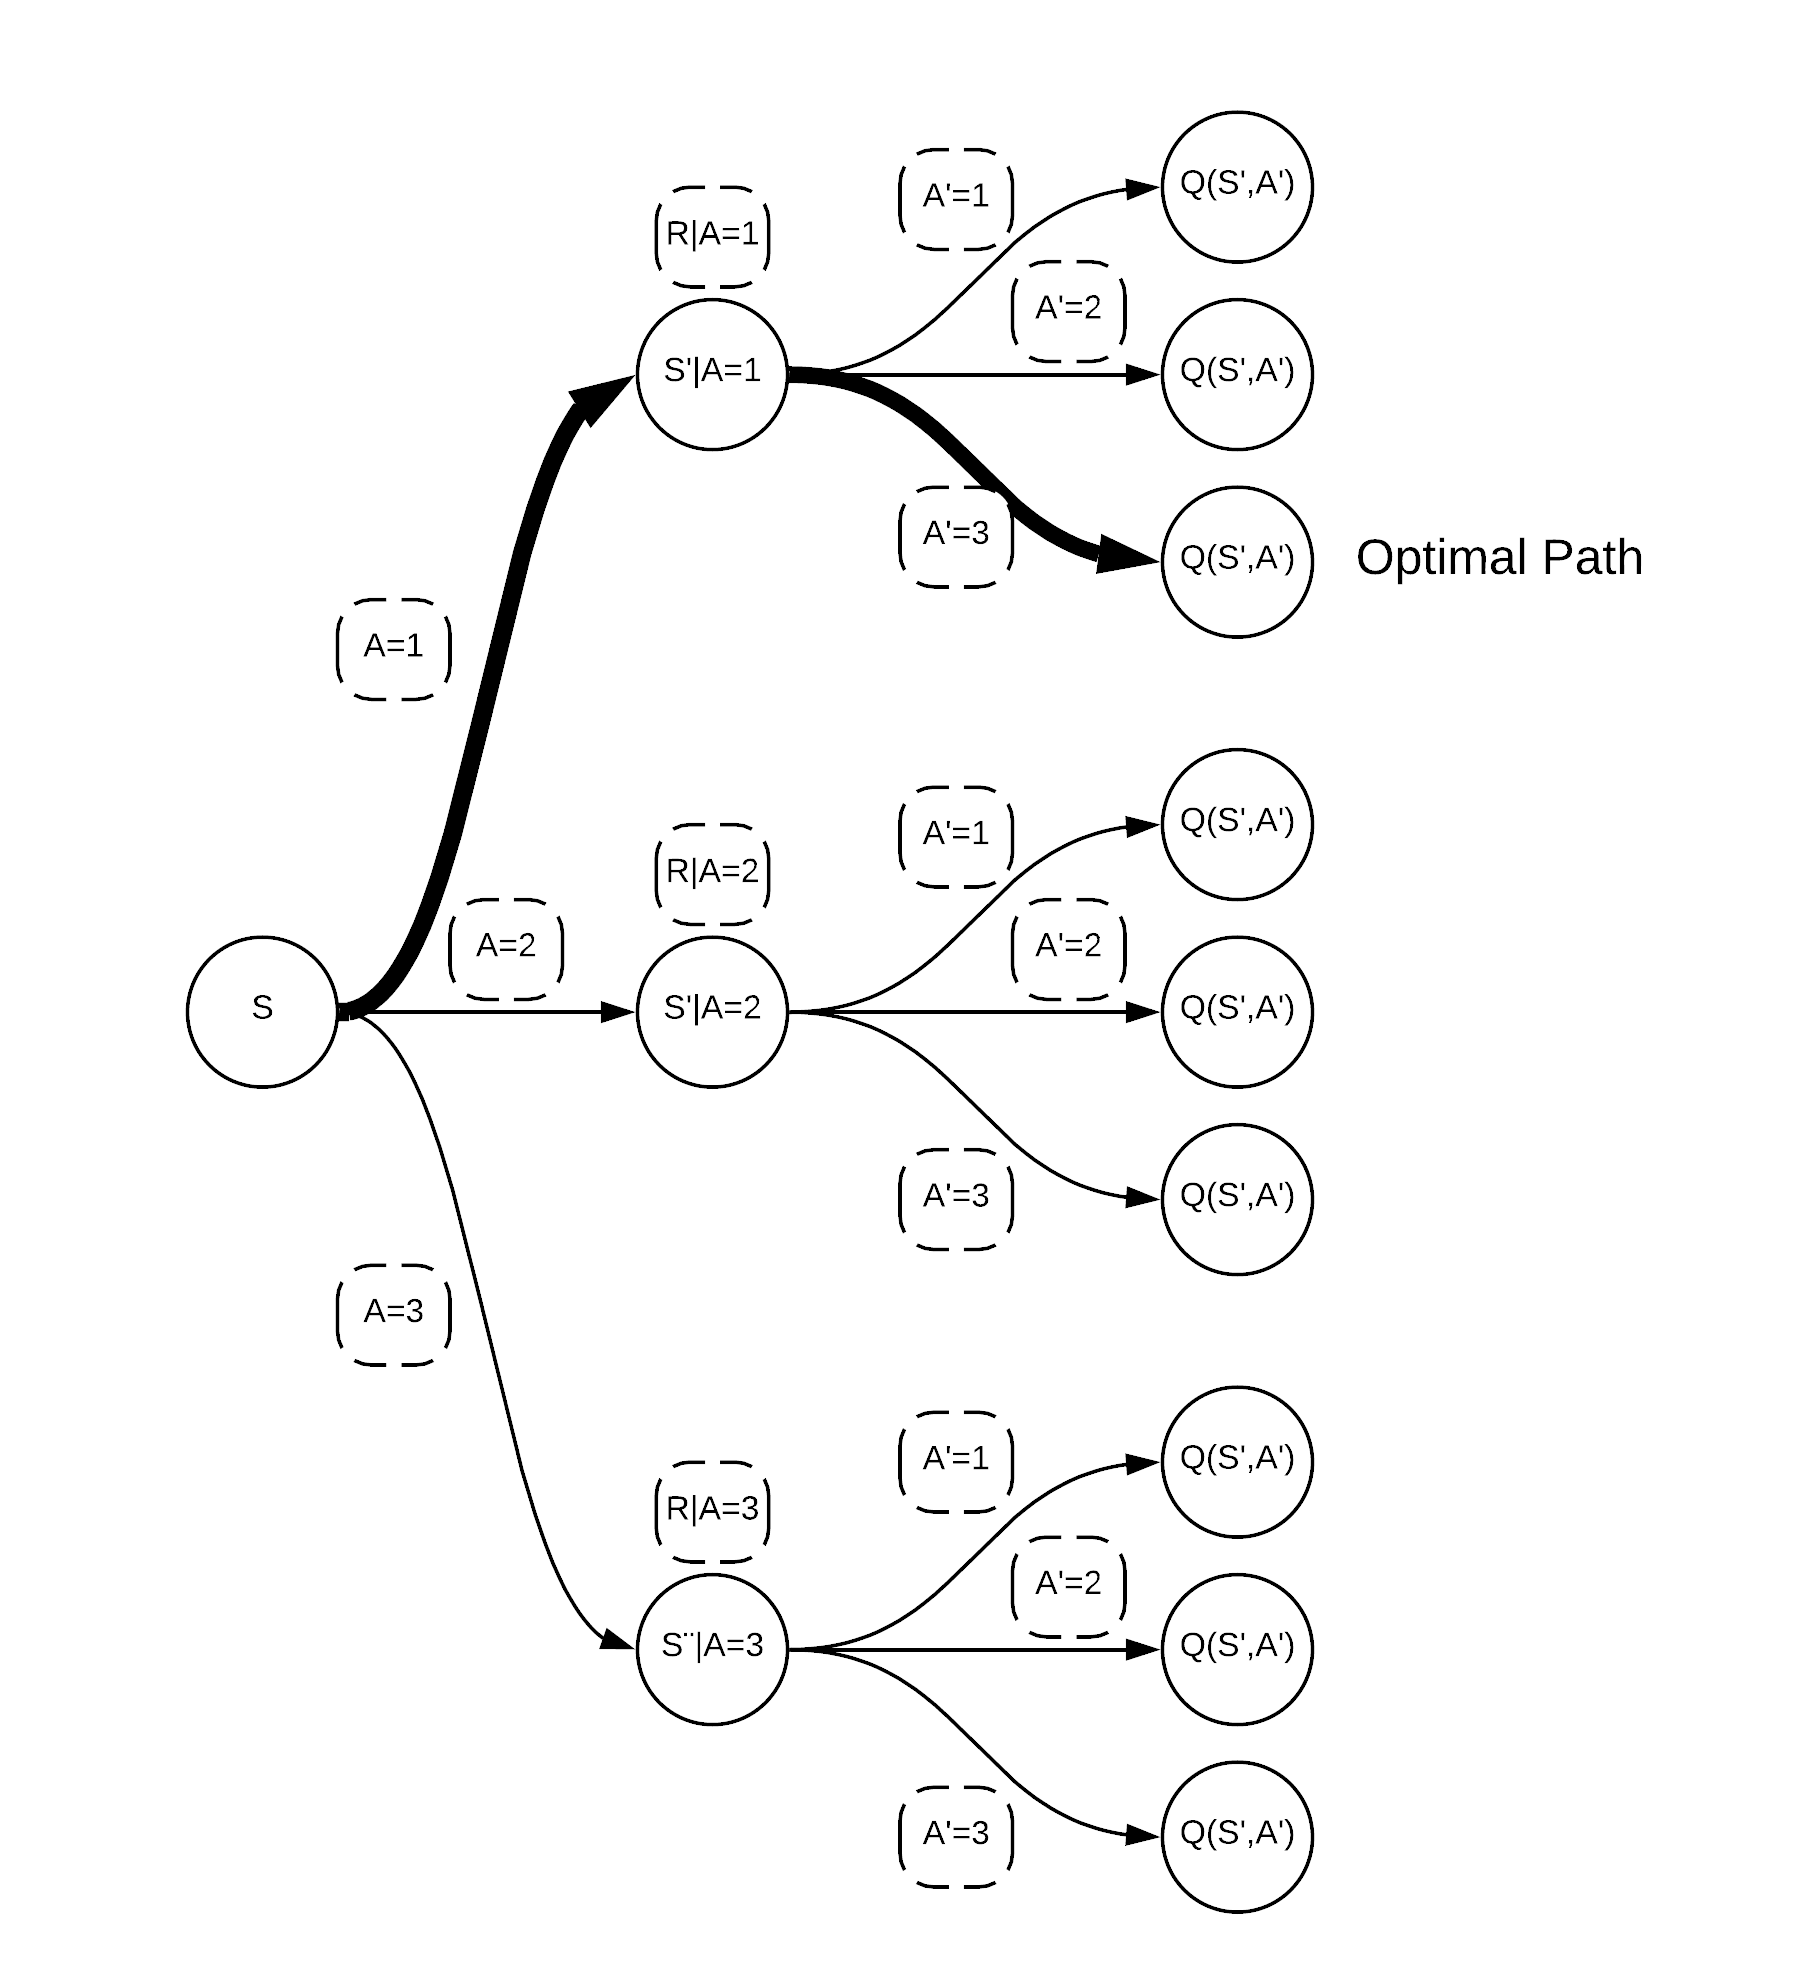
\includegraphics[scale=0.15]{figures/vfi_figure.png}
    \caption{Value function iteration using Q-function}
    \label{fig:vfi_figure}
\end{figure}

The Q-function for each action in the actionspace is made by mapping each $a\in \actionspace$:

\begin{equation}
 Q(S, A=a) = R_t + \gamma \underset{a'\in \actionspace}{\max} Q(S', a')
\end{equation}

In that sense this can be consideread akin to monte carlo integration, however instead of appoximating the expectation in a single point, rather find the distribution of the rewards + discounted value function over the entire state space. The idea is to approximate the integral by using a statistical method, and in this case Deep Learning (another machine learning method would be equally good). Consider $f$ to be a machine learning function, that has the property:

\begin{equation}
    f: \statespace \mapsto\R^{\mid \actionspace \mid}
\end{equation}

For a given point in state space a prediction of the value function is computed for each possible action. This implies the method only is feasible for discrete state space. By trying to reduce the mean squared error between the the true values of the Q-function, and the prediction, the $\E[Q(a, s)]$ can be found, which corresponds to integration as could be done using f.x. Gauss Hermite or Monte Carlo integration.

\begin{algorithm}[H]
\SetAlgoLined
\KwResult{Write here the result }
 Initialize $\tilde{Age} = Age_{max}$\;
 Initialize empty lists for storing results: $X, Y$\;
 Initialize memory counter $j=1$\;
 \While{$\tilde{Age} > Age_{min}$}{
  Draw $\{s_i\}_{i=1}^{i=N}$, where $s_i \sim \statespace \mid Age=\tilde{Age}$ \;
  \ForEach{$s_i$}{
  Create empty array $Z$ of length $\mid \actionspace \mid$\;
  \eIf{$\tilde{Age}= Age_{max}$}{
   \ForEach{$a_k \in \actionspace$}{
    $Z[k] \leftarrow r(s_i, a_k)$ \;
   }
   }{
   \ForEach{$a_k \in \actionspace$}{
    $Z[k] \leftarrow r(s_i, a_k)$ + $\gamma \underset{a' \in \actionspace}{\max}\lsp \hat{q}(a', s_i') \rsp$\;
    }
  }
  $Y[j] \leftarrow Z, X[j] \leftarrow s_i$\;
  $j = j + 1$\;
  }
  Estimate $\hat{Q}$ by training a Deep NN using samples from $X, Y$.
 }
 \caption{Deep Q-function iteration solution method}
 \end{algorithm}

Since i use a deep neural network to approximate the $Q$-function, certain things need to be considered. First and foremost I need to consider the architecture of the network. Next I need to consider the train

For each age i draw 20.000 random samples. This is because any smaller number of draw seemed to be detrimental to the performance. This is inline with standard Deep Learning practices. These kinds of network is known to be very data hungry. When training the network i draw a random sample of 100.000 observations. If I have not yet accumulated 100.000 observations the algorithm draws all observations. The architecture of network is fairly simple being a two-layer fully connected network. First layer being 16 nodes wide, second fully connected layer being 8 nodes wide. I found that mini batching, did not seem to work well on this particular task, and instead i train on all observations, using a validation split of 30 \%, training for a maximum of 150 epochs and finally i allow for early stopping, that is, when the validation loss is not furthering decreasing i stop the training of the network. I do allow the algorithm a patience of 5. Implying that the algorithm will try to lower it's validation loss for five additional epochs before terminating the training.


\begin{figure}[ht]
\begin{subfigure}{.5\textwidth}
  \centering
  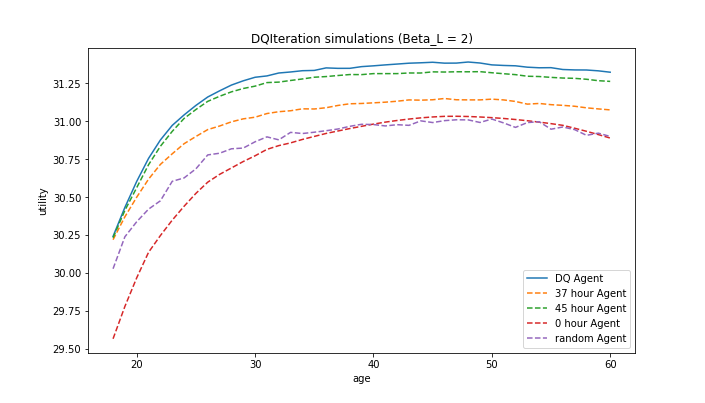
\includegraphics[width=1\linewidth]{figures/dqi_model1_beta_2_solution_benchmark_paths.png}
  \caption{Simulated Paths}
  \label{fig:dqi_solution_beta2_path}
\end{subfigure}%
\begin{subfigure}{.5\textwidth}
  \centering
  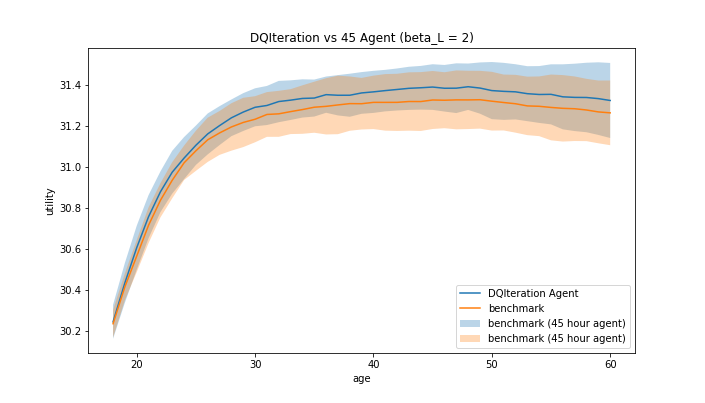
\includegraphics[width=1\linewidth]{figures/dqi_model1_beta_2_solution_benchmark_variance.png}
  \caption{Variance of Paths}
  \label{fig:dqi_solution_beta2_var}
\end{subfigure}
    \caption{Value Function Iteration solution vs. benchmark $(\beta_L = 2)$}
    \label{fig:dqi_solution_beta2}
\end{figure}

\begin{figure}[ht]
\begin{subfigure}{.5\textwidth}
  \centering
  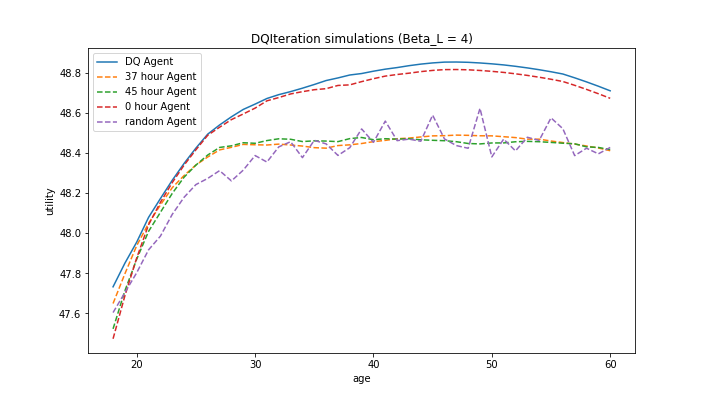
\includegraphics[width=1\linewidth]{figures/dqi_model1_beta_4_solution_benchmark_paths.png}
  \caption{Simulated Paths}
  \label{fig:dqi_solution_beta4_path}
\end{subfigure}%
\begin{subfigure}{.5\textwidth}
  \centering
  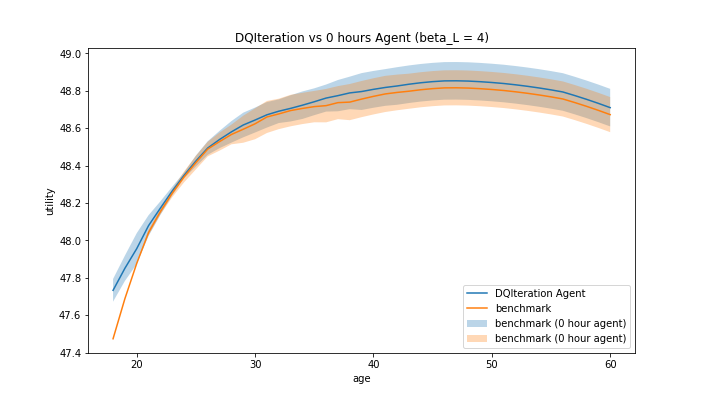
\includegraphics[width=1\linewidth]{figures/dqi_model1_beta_4_solution_benchmark_variance.png}
  \caption{Variance of Paths}
  \label{fig:dqi_solution_beta4_var}
\end{subfigure}
    \caption{Value Function Iteration solution vs. benchmark $(\beta_L = 4)$}
    \label{fig:dqi_solution_beta4}
\end{figure}

Figure \ref{fig:dqi_solution_beta2} and \ref{fig:dqi_solution_beta4} shows the results of the Value Function Iteration algorithm\footnote{The plots use the name DQIteration (Deep Q-Function Iteration) instead of Value Function Iteration.} compared to 4 benchmarks. Three deterministic agents working either $0$, $37$ or $45$ hours pr. week and one agent taking random actions. Figure \ref{fig:dqi_solution_beta2} shows the utility for each step over the life cycle when the preference for leisure is fixed at $\beta_L = 2$. As the figure shows the DQ Agent (VFI agent) learns to navigate the environment, just as well as the best deterministic agent. Looking to the right hand side plot of \ref{fig:dqi_solution_beta2} it's clear that there is a great overlap between the two agents. The variance of the path is represented as one standard deviation of the utility for a given age for all episodes of the given agent. Figure \ref{fig:dqi_solution_beta4} compares the benchmark agents with the VFI solution when considering a preference for leisure $\beta_L = 4$. Again the VFI solution is as good as the best benchmark.

\newpage

\subsection{Deep Q-learning}

In this paper I implement the algorithm used by \parencite{mnih_playing_nodate} for beating Atari games as a way to solve model. First note here, however few modifications will be made to the original implementation, due to the fact, the environment they were only using sensory data (an RGB representation of an image), where a part of their achievement was to transform these images into features that which the value function accurately could map into scores of the game. 

Just as described in section \ref{sec:rl_theory} the algorithm tries to maximize the Bellman equation. However now the value-function is estiamted using Deep neural network as a function approximator. Mathematically this can be described as finding:

\begin{equation}
    Q^*(s_t,a_t) = \E [r_t + \underset{a_{t+1}}{\max}  Q^*(s_{t+1}, a_{t+1}) \mid s_t, a_t]
\end{equation}

However here $Q^*(s, a)$ is approximated by a parametric function (in this case a Deep Neural Network) $Q(s, a ; \theta)$. Folloing the terminology of \parencite{mnih_playing_nodate}, this function approximator is referred to as the Q-network. This Q-network can be trained using stochastic gradient descent as described in section \ref{sec:deep_learning}:

\begin{equation}
    \Loss_i(\theta_i) = \E \lsp (y_i - Q(s_t, a_t ; \theta_i))^2 \rsp
\end{equation}

where:

\begin{equation}
    y_i = \E [r_t + \gamma \underset{a_{t+1}}\max Q(s_{t+1}, a_{t+1}; \theta_{i-1}) \mid s_t, a_t ]
\end{equation}

where $i$ implies the iteration of the algorithm, such $i$ increments by one for each update of the parameters $\theta$. This implies the update equation determining the update:

\begin{equation}
    \nabla_{\theta_i} \Loss_i (\theta_i)  \E \lsp \lp y_i - Q(s_t, a_t ; \theta) \rp \nabla_{\theta_i} Q(s_t, a_t; \theta_i) \rsp
\end{equation}

Where i follow the formulation of \parencite{mnih_playing_nodate} that $Q(s_{t+1}, a_{t+1}; \theta_{i-1})$ is held fixed, allowing for just writing $y_i$, and not the parametric form of $y_i$.

A traditional choice would be to update the weight after each step in the algorithm only using the last sample. This would the correspond to the traditional Q-learning algorithm. This was the approach used in by to create the TD Gammon created by Tesauro\footnote{I have not been able to get acces to the original paper, so I have relied on the description made by Sutton and Barto.} as described by \parencite{sutton_reinforcement_2018}. However, this approach of using Q-learning with a non-linear function approximator has been shown to diverge, and did not extend itself well to learning any other game than backgammon \parencite{tsitsiklis_analysis_1997}. To accommodate this problem a replay buffer is implemented. At each step in a entry is made to the replay memory containing $s_t, a_t, r_t, s_{t+1}$. This data set $\mathcal{D}$ has a capacity of $N$ entries. Using this replay memory a random sample (mini batch) is drawn used to update the weights of the Q-network. Note here that the capacity of the memory buffer should be greater, by a substantial margin than the number of samples drawn. The random sample has a couple of advantages. It has decorelated observations to update the weights on, allowing for better training \parencite{mnih_playing_nodate}. Using a replay buffer requires off-policy learning which is the reason for using Q-learning. This is due to the fact that current parameters $\theta$ is not the same as those generating the data. Note that experiences is drawn randomly, and no experiences (which could have important insights) is prioritized. The full algorithm is summarized below in algorithm \ref{alg:dqlearning}.

\begin{algorithm}[H]
\SetAlgoLined
 Initialize replay memory $\mathcal{D}$ with capacity $N$\;
 Initialize action-value function $Q$ with random weights\;
 Initialize memory counter $j=1$\;
 \ForEach {episode $\in \{1, 2, \cdots M \}$}{
  Initialize sequence with an initial state $s_1$. This is drawn randomly.\;
    \For{$t \in \{1, 2, \cdots, T \}$}{
    With probability $\epsilon$ select a random action $a_t$\;
    Otherwise select $a_t = \underset{a_t}{\argmax}Q^*(s_t, a_t ; \theta)$\;
    Execute action $a_t$ in environment and observe reward $r_t$ and the new state $s_{t+1}$\;
    Store transition $(s_t, a_t, r_{t+1}, s_{t+1})$ in $\mathcal{D}$\;
    Sample random mini-batch of transitions $(s_t, a_t, r_{t+1}, s_{t+1})$ from $\mathcal{D}$\;
    Set $
      y_j = \begin{cases}
        r_j & \text{if terminal states} \\
        r_j + \gamma \underset{a_{t+1}}{\max}Q(s_{t+1}, a_{t+1}; \theta) & \text{if non-terminal states}
      \end{cases}
    $ \;
    Perform gradient descent step on $(y_j - Q(s_t, a_t ; \theta))^2$ \;
    Increment $j$\;
  }
}
\caption{Deep Q-learning}
\label{alg:dqlearning}
\end{algorithm}

Just as \parencite{mnih_playing_nodate} this implementation has the following trock to reduce the number of computations needed. The Q-function maps a state action pair to a scalar value estimates of the Q-value, the most obvious implementation would let the action be part of the input to the function. However, such implementation would require $\actionspace$ number of look ups, at each step, since each action in the action space must be used for evaluation. Instead the Q-function maps the state space to a scalar value for each action, just as described in section \ref{sec:rl_theory}: $Q: \statespace \mapsto \R^{\mid \actionspace \mid}$. 

The solutions used the following hyper parameters and architecture decisions: The Deep Neural network consists of an input layer (size of state space). Then  2 fully connected layers of width $256$ using rectified linear units as activation functions. Finally the network uses a linear output layer for its predictions. The output layer is of the same size as the action space. The learning rate, $\alpha=0.0005$ and I let epsilon be decremented after each update by: $\epsilon_i = \max (\epsilon_{i-1} \cdot 0.9999, 0.01$), where $0.01$ is the minimum exploration that can be done. The replay buffer has a capacity of 1 million rows, and the mini batches used for updating the parameters is $64$ rows. I scale the state space so that each row variable approximately has mean zero and standard deviation of 1 when doing the batch training. This helps performance, and in general accepted as being an important step for getting good performance out of neural networks \parencite{goodfellow_deep_2016}. The impatience parameter is set to $\gamma=0.99$, using a standard value. I make the parameter $\beta_L$ a part of the state space, drawing a random value (uniformly) in the interval $[0.2, 6.0]$ at the beginning of each episode, letting the agent navigate through the environment with given preference for leisure. This is done, so only a single solution of the model is necessary for estimating the parameter later. I scale the rewards (so they are approximate zero mean and have a standard deviation of 1, conditional on the $\beta_L$ value. Again this is done to improve the training performance and to do introspection; it becomes possible to see if there is any trend in the training performance. The algorithm is trained for 3000 episodes. Figure \ref{fig:training_performance_simple_model}  (left plot) shows the training performance of the Deep Q-learning algorithm. The plot shows the cumulative rewards over the life cycle of the agents for each episode. The performance begins at around 2.5 and ends at an average of $7.9$ as the asymptotic value. The performance seems to reach this asymptotic level at around 1000 episodes. I use the Adam optimizer for the gradient descent step when updating the weights.

\begin{figure}[ht]
\begin{subfigure}{.5\textwidth}
  \centering
  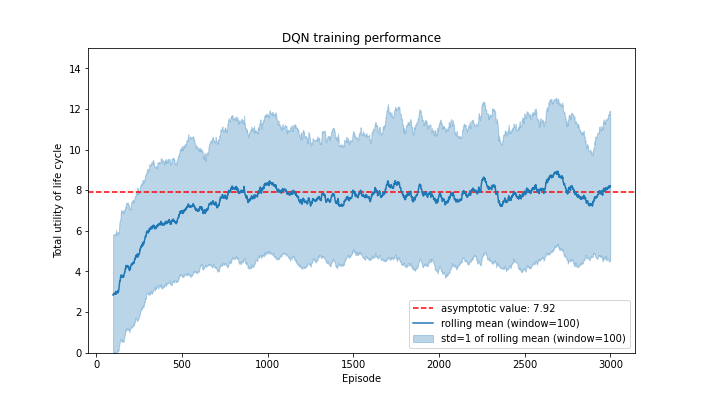
\includegraphics[width=1\linewidth]{figures/dqn_training_performance_simple_model.png}
  \caption{DQN Training Performance}
  \label{fig:dqn_training_performance_simple}
\end{subfigure}%
\begin{subfigure}{.5\textwidth}
  \centering
  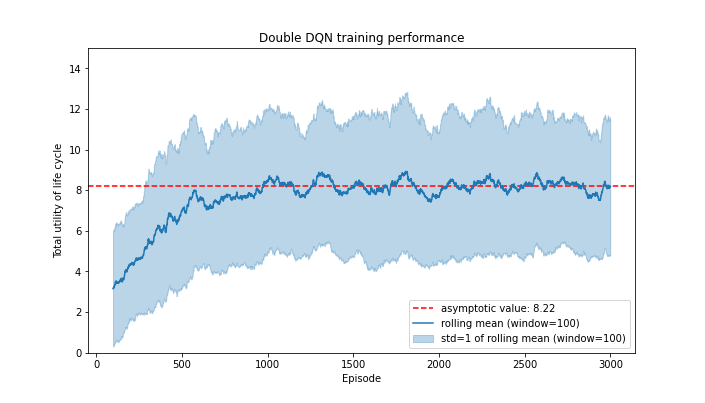
\includegraphics[width=1\linewidth]{figures/ddqn_training_performance_simple_model.png}
  \caption{Double DQN Training Performance}
  \label{fig:ddqn_training_performance_simple}
\end{subfigure}
    \caption{Comparing training perfance of Deep Q-Learning and Double Deep Q-Learning}
    \label{fig:training_performance_simple_model}
\end{figure}

Figure \ref{fig:dqn_solution_beta2} and \ref{fig:dqn_solution_beta4} compares the performance of the algorihtm to two different benchmarks. One benchmark is the when the $\beta_L = 2$ another $\beta_L=4$. These differences in preferences will yield different optimal policies conditional on the $\beta_L$. I compare the policy chosen by the agent with different deterministic policies. Figure \ref{fig:dqn_solution_beta2} (left plot) shows either using $0, 37, 45$ hours pr. week as comparisons and an agent picking randomly. All agents have been simulated for 300 episodes, yielding the plots being averages, and the standard deviations are calculated on an age basis for each agent. It should also be noted that $\epsilon$ (the exploration ratio of the agent) is set to 0, such that the agent now only greedily explores the environment. Comparing this to the DQN agent I find that it's reasonable to assume that the DQN agent has learned to navigate the environment. A small dip from around age 55 can be observed, but I believe this does not make the feat any less impressive, and furthermore I believe that the solution fairly accurately approximates the correct optimal policy. Looking to the the right hands side plot, the variance of the utility (1 standard deviation). Again the best benchmark for $\beta_L = 2$ an agent that works 45 hours a week, seem have a overlap even in the last periods, where they diverge a little, allowing me to conclude, that this differences in performance is very small. Figure \ref{fig:dqn_solution_beta4} shows the same plot just for $\beta_L = 4$. Again the DQN agent fairly accurately approximates the optimal policy, with even less variance than observed in with $\beta_L = 2$. One thing to note is, that a small hump can be observed for the DQN agent at around age 28, where it has found a way to beat the deterministic policy. Again this might just be variance of the simulations. 


\begin{figure}[ht]
\begin{subfigure}{.5\textwidth}
  \centering
  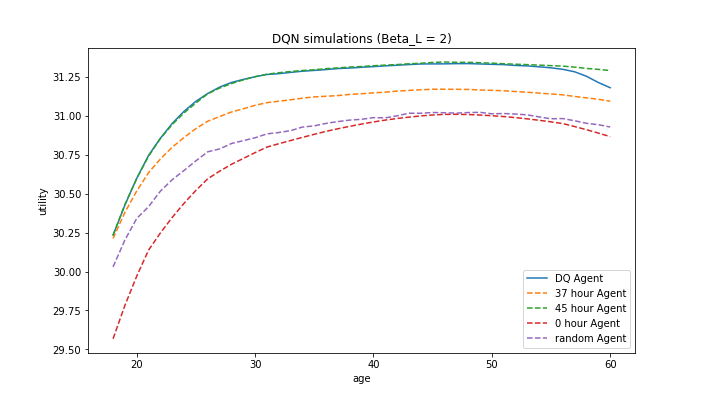
\includegraphics[width=1\linewidth]{figures/dqn_model1_beta_2_solution_benchmark_paths.png}
  \caption{Simulated Paths}
  \label{fig:dqn_solution_beta2_path}
\end{subfigure}%
\begin{subfigure}{.5\textwidth}
  \centering
  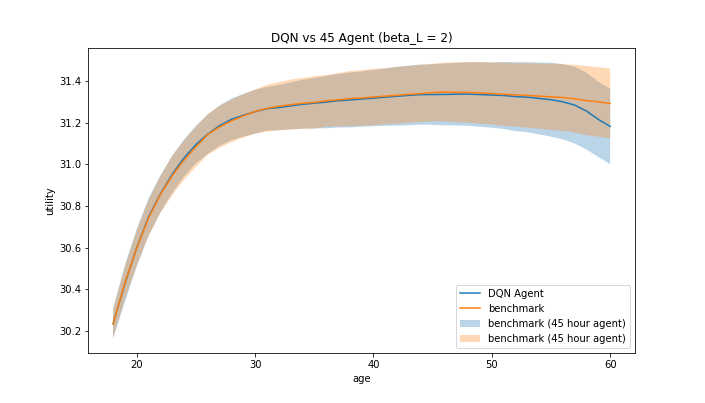
\includegraphics[width=1\linewidth]{figures/dqn_model1_beta_2_solution_benchmark_variance.png}
  \caption{Variance of Paths}
  \label{fig:dqn_solution_beta2_var}
\end{subfigure}
    \caption{Deep Q-Learning solution vs. benchmark $(\beta_L = 2)$}
    \label{fig:dqn_solution_beta2}
\end{figure}

\begin{figure}[ht]
\begin{subfigure}{.5\textwidth}
  \centering
  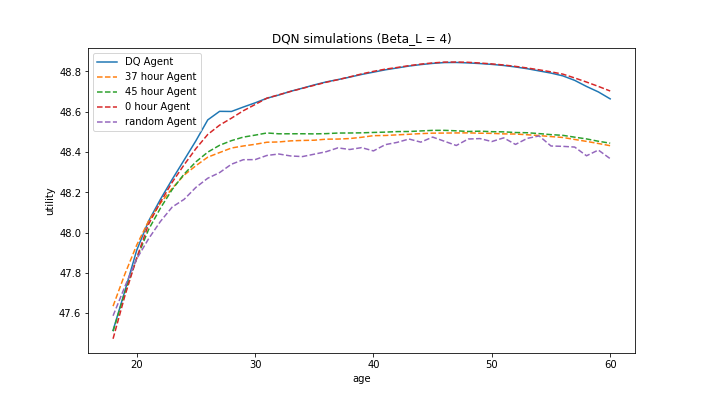
\includegraphics[width=1\linewidth]{figures/dqn_model1_beta_4_solution_benchmark_paths.png}
  \caption{Simulated Paths}
  \label{fig:dqn_solution_beta4_path}
\end{subfigure}%
\begin{subfigure}{.5\textwidth}
  \centering
  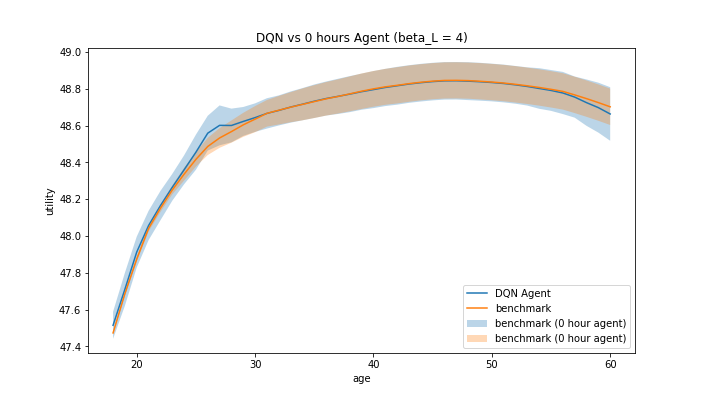
\includegraphics[width=1\linewidth]{figures/dqn_model1_beta_4_solution_benchmark_variance.png}
  \caption{Variance of Paths}
  \label{fig:dqn_solution_beta4_var}
\end{subfigure}
    \caption{Deep Q-Learning solution vs. benchmark $(\beta_L = 4)$}
    \label{fig:dqn_solution_beta4}
\end{figure}


\subsection{Double Deep Q-learning}

Deep Q-learning is good starting point for an learning algorithm using non linear function approximation, however certain properties of the algorithm is problematic. This is mainly due to the fact that Deep Q-learning can tend to be overoptimistic, and that in a problematic way \parencite{van_hasselt_deep_2015}. In general there exists two ways in which overoptimism can be good or at least not detrimental to performance. 1) If the algorithm uniformly overestimates the Q-function for all actions, then this is not associated with any problems, since then taking the max over the action, will lead to the same result had the estimations been correct. In other words performance would not change, however introspection of the algorithm might be harder. 2) It can be a good thing for an algorithm to be optimistic when faced with uncertainty. If an action would lead to observing an unexplored part of the state space, it might be a good thing to be optimistic with regards to exploration, allowing for possible new policies with higher yielding returns over the episode. Deep Q-learning however does not adhere to any of these properties, instead it usually overestimates the value of the action it has taken due to the max operator in the value estimation: $R_{t+1} + \gamma \underset{A_{t+1}}{\argmax} Q(S_{t+1}, A_{t+1})$. An simple extension \parencite{van_hasselt_deep_2015} is to de-couple the prediction with the evaluation. This can be done by having two different sets of weights $\theta$ and $\tilde{\theta}$, where one is used for evaluation and one is used for the policy. This can be presented the following way. The Q-network target:

\begin{equation}\label{eq:dqn_target}
    Y_t^{Q} = R_{t+1} + \gamma Q(S_{t+1}, \underset{a}{\argmax} (S_{t+1}, a ; \theta) ; \theta)
\end{equation}

and the Double DQN target is calculated:

\begin{equation}\label{eq:ddqn_target}
    Y_t^{DoubleQ} = R_{t+1} + \gamma Q(S_{t+1}, \underset{a}{\argmax}Q(S_{t+1}, a; \theta); \tilde{\theta}) 
\end{equation}

This alleviates the problem of overestimating the values taking by the algorithm for the following reason. Consider \eqref{eq:dqn_target}. When calculating the value of the state action pair, one uses the same function to choose the action (through the $\argmax$ operator, which can cause the overestimation of the state action pair of the chosen action. The equation below \eqref{eq:ddqn_target} instead estimates the value of the position by using a different set of parameters, $\tilde{\theta}$. Following the implementation of \parencite{van_hasselt_deep_2015} instead of training 2 separate networks instead, which would be perfectly decouple, to reduce time one of the network simply inherits the old weights. Which imply $\tilde{\theta} = \theta^{previous}$. Such that, the target estimation is made by the old weights, while the value of greedy policy uses the new weights:

\begin{equation}\label{eq:ddqn_target_final}
    Y_t^{DoubleQ} = R_{t+1} + \gamma Q(S_{t+1}, \underset{a}{\argmax}Q(S_{t+1}, a; \theta_t); \theta_t^{previous}) 
\end{equation}

The full algorithm, which to large extend mirrors the algorithm for Deep Q-learning is as follows, is presented in algorithm \ref{alg:ddqlearning}:

\begin{algorithm}[H]
\SetAlgoLined
 Initialize replay memory $\mathcal{D}$ with capacity $N$\;
 Initialize action-value function $Q$ with random weights: $\theta, \tilde{\theta}$\;
 Initialize memory counter $j \leftarrow 1$\;
 Initialize $k$ when to replace target weights $\tilde{\theta}$\;
 \ForEach {episode $\in \{1, 2, \cdots M \}$}{
  Initialize sequence with an initial state $s_1$. This is drawn randomly.\;
    \For{$t \in \{1, 2, \cdots, T$}{
    With probability $\epsilon$ select a random action $a_t$\;
    Otherwise select $A_t = \underset{a}{\argmax}Q^*(S_t, A_t ; \theta)$\;
    Execute action $A_t$ in environment and observe reward $R_t$ and the new state $S_{t+1}$\;
    Store transition $(S_t, A_t, R_{t+1}, S_{t+1})$ in $\mathcal{D}$\;
    Sample random mini-batch of transitions $(S_t, A_t, A_{t+1}, S_{t+1})$ from $\mathcal{D}$\;
    Set $
      Y_j = \begin{cases}
        R_j & \text{if terminal states} \\
        R_j + \gamma Q(S_{t+1}, \underset{a}{\argmax} (Q_t, S_{t+1}; \theta_t); \tilde{\theta_t}) & \text{if non-terminal states}
      \end{cases}
    $ \;
    Perform gradient descent step on $(Y_j - Q(S_t, A_t ; \theta))^2$ w.r.t $\theta$ \;
    If $j$ is divisible by $k$ replace target weights $\tilde{\theta} \leftarrow \theta$\;
    Increment $j$ \;
  }
}
\caption{Double Deep Q-learning}
\label{alg:ddqlearning}
\end{algorithm}

Just as with the Deep Q-learning implementation i let the Q-function map from: $\statespace \mapsto \R^{\mid \actionspace \mid}$, to reduce the number of computations, when taking the max over the Q-function. 


For the Double DQN agent I in general use the same hyper parameters used for the DQN agent: The network architecture is again an input layer of the size of the state space, followed by two fully connected layers with Rectified Linear units as activation functions ending with an output layer with linear activation of same size as the action space. Again i let the learning rate be $\alpha = 0.0005$ and the $\epsilon_i = \max (\epsilon_{i-1} \cdot 0.9999, 0.01)$, such that exploration is performed through out the training period. Again the replay buffer has a capacity of a million rows and i use mini batches of size 64 to perform stochastic gradient descent on the weight of the neural network approximating the Q-function. I transform the states such that they are mean zero and a standard deviation of 1. The same is true for the rewards conditional on the $\beta_L$ value. The $\beta_L$ value is just as with $DQN$ and value function iteration added to the state space, allowing for a single solution of the model. I uniformly draw $\beta_L$ from the interval $[0.2, 6]$ and sets this to be part of the environment in the beginning of each episode. When using gradient descent on the weights I use the Adam optimizer. I let the target network inherit the old weights every 100'th iteration of the algorithm. The algorithm is trained for 3000 episodes. Figure \ref{fig:training_performance_simple_model} (right plot) shows the performance. Very similar to the DQN I find that the performance stabilized at around 1000 episodes, and reaches an asymptotic performance of $8.22$, which is slightly higher compared to the DQN agent which had an asymptotic value of $7.92$.

\begin{figure}[ht]
\begin{subfigure}{.5\textwidth}
  \centering
  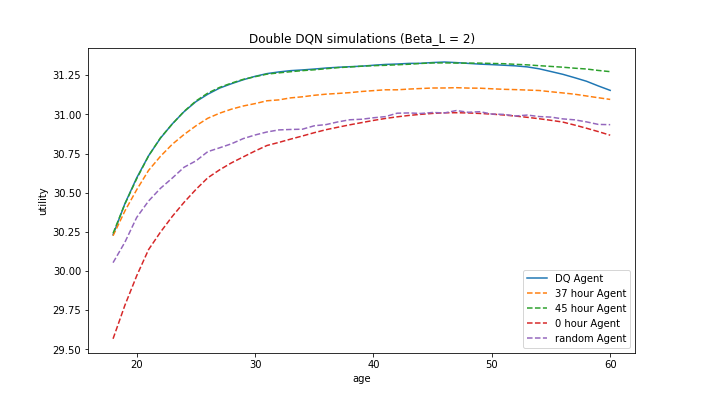
\includegraphics[width=1\linewidth]{figures/ddqn_model1_beta_2_solution_benchmark_paths.png}
  \caption{Simulated Paths}
  \label{fig:ddqn_solution_beta2_path}
\end{subfigure}%
\begin{subfigure}{.5\textwidth}
  \centering
  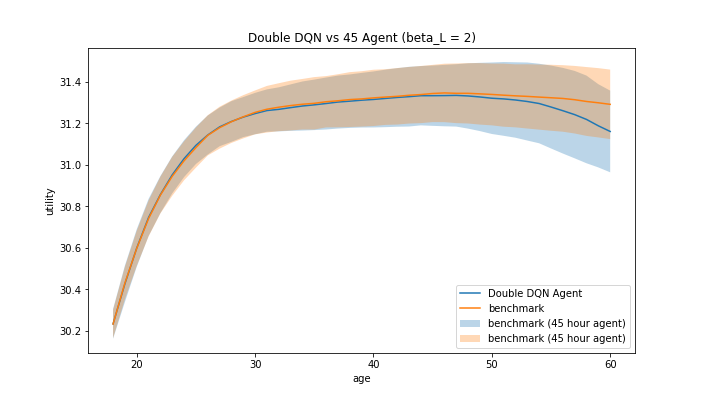
\includegraphics[width=1\linewidth]{figures/ddqn_model1_beta_2_solution_benchmark_variance.png}
  \caption{Variance of Paths}
  \label{fig:ddqn_solution_beta2_var}
\end{subfigure}
    \caption{Double Deep Q-Learning solution vs. benchmark $(\beta_L = 2)$}
    \label{fig:ddqn_solution_beta2}
\end{figure}

\begin{figure}[ht]
\begin{subfigure}{.5\textwidth}
  \centering
  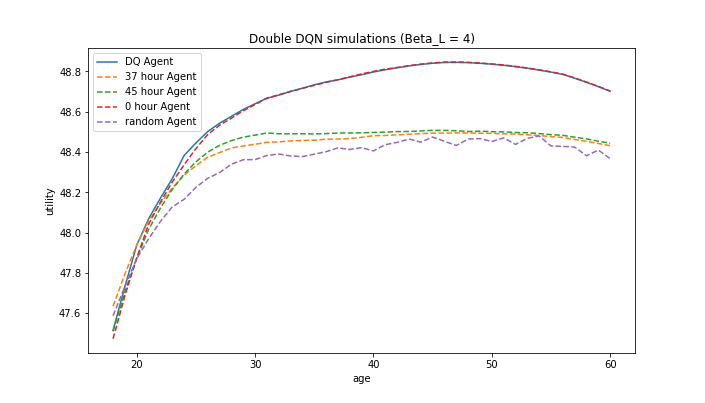
\includegraphics[width=1\linewidth]{figures/ddqn_model1_beta_4_solution_benchmark_paths.png}
  \caption{Simulated Paths}
  \label{fig:ddqn_solution_beta4_path}
\end{subfigure}%
\begin{subfigure}{.5\textwidth}
  \centering
  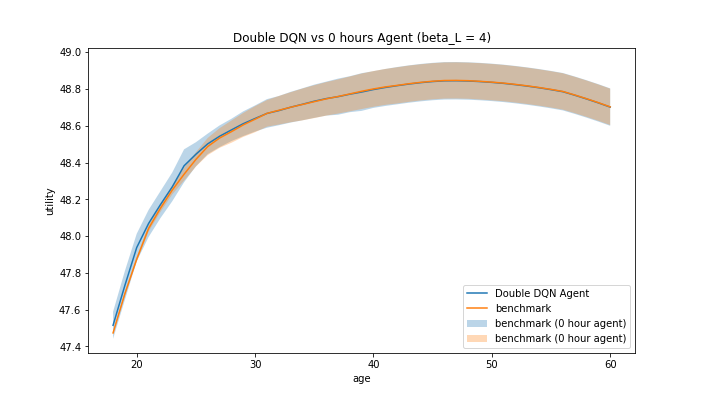
\includegraphics[width=1\linewidth]{figures/ddqn_model1_beta_4_solution_benchmark_variance.png}
  \caption{Variance of Paths}
  \label{fig:ddqn_solution_beta4_var}
\end{subfigure}
    \caption{Double Deep Q-Learning solution vs. benchmark $(\beta_L = 4)$}
    \label{fig:ddqn_solution_beta4}
\end{figure}

Figure \ref{fig:ddqn_solution_beta2} and \ref{fig:ddqn_solution_beta4} shows the performance of the Deep DQN agent comparing it to two different preferences of leisure: $\beta_L = 2$ and $\beta_L = 4$. Four agents is used for comparison: An agent that chooses actions randomly, and three agents that in an deterministic fashion works $0, 37$ or $45$ hours a week. The results of the Double DQN agent is comparable to those found within the other agents (VFI and DQN). Figure \ref{fig:ddqn_solution_beta2} shows the performance where the preference for leisure $\beta_L = 2$. Again the best deterministic policy is the 45 hour agent, which is very close to what the DQ agent chooses, except for the last 5 years of the agent's life cycle where the utility is slightly lower. Comparing the variance of the utility on right hand side plot of figure \ref{fig:ddqn_solution_beta2}, there is overlap of the simulations of the Double DQN agent and the 45 hours a week agent. Figure \ref{fig:ddqn_solution_beta4} compares the Deep DQN agent to the agents when the preference for leissure $\beta_L = 4$. Here again the optimal policy pretty closely mirrors the best deterministic agent, the one which does not work, with a clear overlap presented in figure on right hand side.
